\section{Análisis de objetivos y metodología}

En este apartado se detallarán los aspectos previos a la resolución del proyecto: los objetivos y herramientas a utilizar para resolverlo, así como el uso de una cámara que servirá para obtener imágenes con las que entrenar el modelo clasificador.

\subsection{Objetivos del proyecto}

Como hemos visto, es común en el ámbito del \textit{deep learning} el uso de un dataset ``precocinado'' a la hora de obtener un modelo clasificador. Sin embargo, en problemas reales, el uso de un dataset de estas características no siempre es efectivo ya que acostumbran a adoptar un enfoque generalista en cuanto a distribución de clases.

El caso que nos ocupa es el \textit{tracking} de un balón en un partido de volleyball, con la peculiaridad de que se utilizará solamente una cámara con una vista cenital sobre el campo (figura \ref{fig:campo}), a diferencia de otros productos comerciales donde se llega a utilizar hasta 38 cámaras como hemos visto.

Usando imágenes de esta cámara, la meta es lograr un dataset de suficiente calidad como para entrenar un modelo de red neuronal que permita identificar el balón en la escena desde 0. Para ello, deberán extraerse imágenes de los vídeos de la cámara, para su posterior etiquetado como imágenes con balón o sin él, cuidando la limpieza del dataset así como su calidad.

Una vez obtenido un dataset, se entrenará un modelo que clasifique la presencia o ausencia de balón en dichas imágenes. Idealmente (suponiendo un clasificador perfecto) deberíamos ser capaces de seguir el balón durante la totalidad del vídeo sin utilizar ningún modelo de consistencia temporal.

Un posible problema a considerar es la velocidad que puede llegar a alcanzar el balón durante situaciones normales de juego, donde llega a convertirse casi en un borrón en el vídeo. También deberemos tener en cuenta el problema de las oclusiones, donde un detector desde 0 sin nada de consistencia temporal va a presentar con mayor probabilidad problemas en la detección.

\begin{figure}
    \centering
    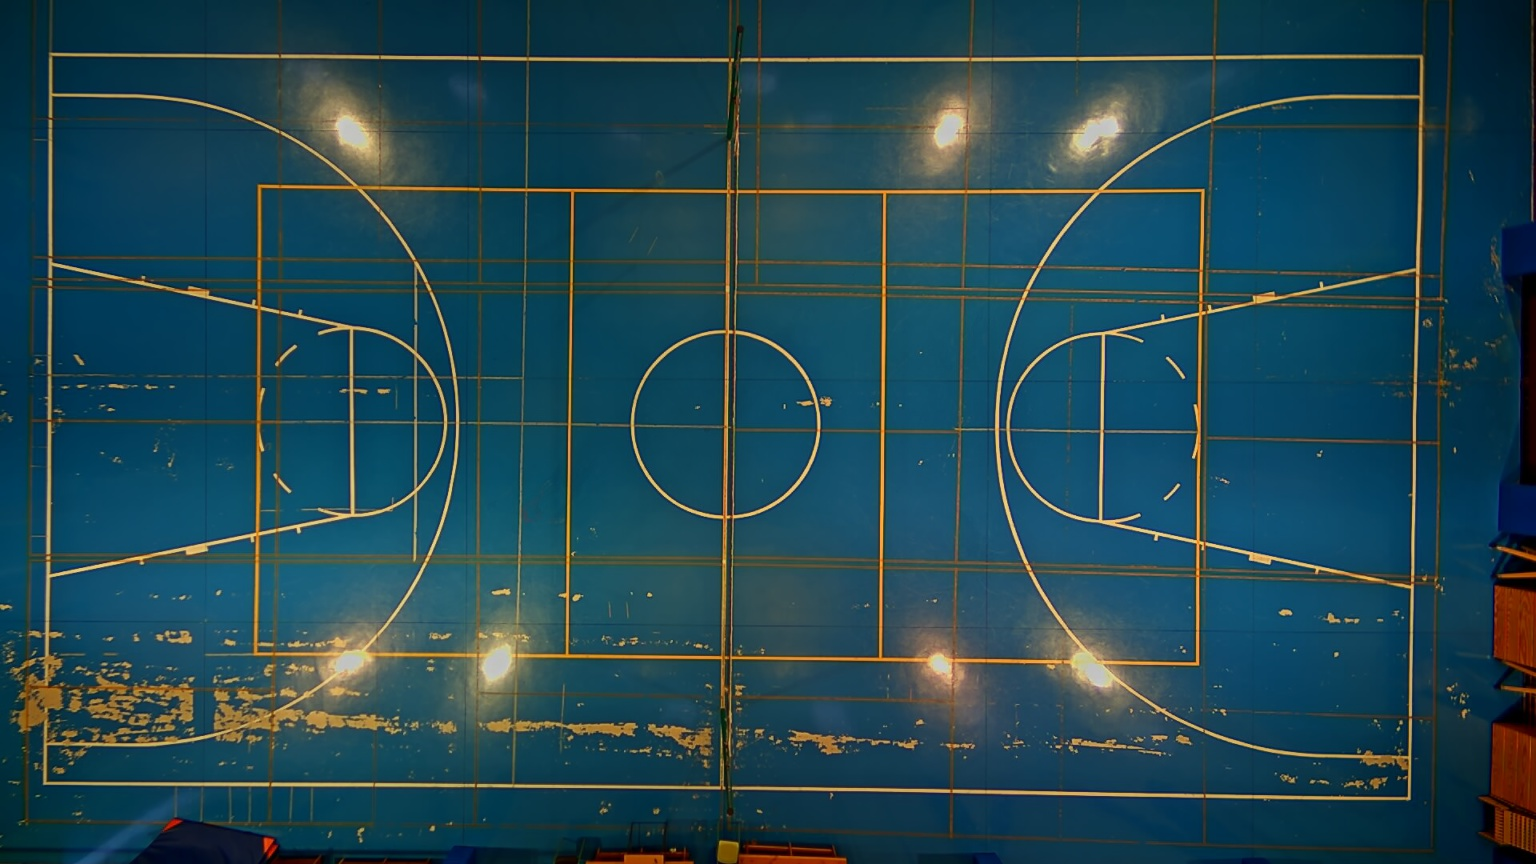
\includegraphics[width=0.6\textwidth]{images/campo}
    \caption{Imagen del campo vacío.}
    \label{fig:campo}
\end{figure}

\subsection{Instalación de cámara en el pabellón}
En el desarrollo de este proyecto se han utilizado imágenes de una cámara instalada con anterioridad en el desarrollo de mi TFG. Dicha cámara es un modelo AXIS P1365-E Mk II (figura \ref{fig:camara}), cuyas características, según su ficha técnica, son:

\begin{figure}
    \centering
    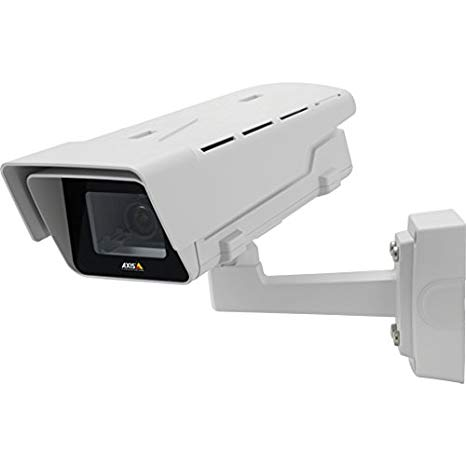
\includegraphics[width=0.5\textwidth]{images/camara}
    \caption{Imagen de la cámara AXIS P1365-E Mk II.}
    \label{fig:camara}
\end{figure}

\begin{itemize}
    \item Rango de temperaturas operativas entre -40 ºC y 50 ºC.
    \item Resistencia a impactos.
    \item Uso de la tecnología Zipstream, que reduce el ancho de banda necesario para el envío del vídeo.
    \item Vídeo a 1080p y hasta 60 fps.
\end{itemize}

En este caso, la cámara graba a 1080p y 30fps, con un ancho de banda de 100 Mbps en la transferencia de vídeo. Se conecta mediante Power over Ethernet (PoE). El objetivo de la cámara cuenta con zoom óptico variable, con un \textit{field of view} entre 35-107º en horizontal y 19-67º en vertical. Usando el fov máximo y considerando los dos triángulos rectángulos formados por la vertical de la cámara, el campo y el ángulo de apertura de esta:
\[
    2 \cdot \tan(\frac{107}{2} \cdot \frac{\pi}{180}) = 2.70
\]
de lo que se deduce que el rango de metros visibles en horizontal es de $2.7\cdot altura_{cam}$. El techo del pabellón es de 10,1 metros, con lo cual el rango máximo de la cámara es de 27,27 metros. En vertical, usando la misma fórmula, el rango máximo es de $1.3 \cdot altura_{cam}$, lo que nos da 13,13 metros de rango vertical. Dado que el tamaño oficial de una pista de volley es 18x9 metros, el rango de visión que tenemos es más que suficiente.

\begin{figure}
\begin{subfigure}{.5\textwidth}
  \centering
  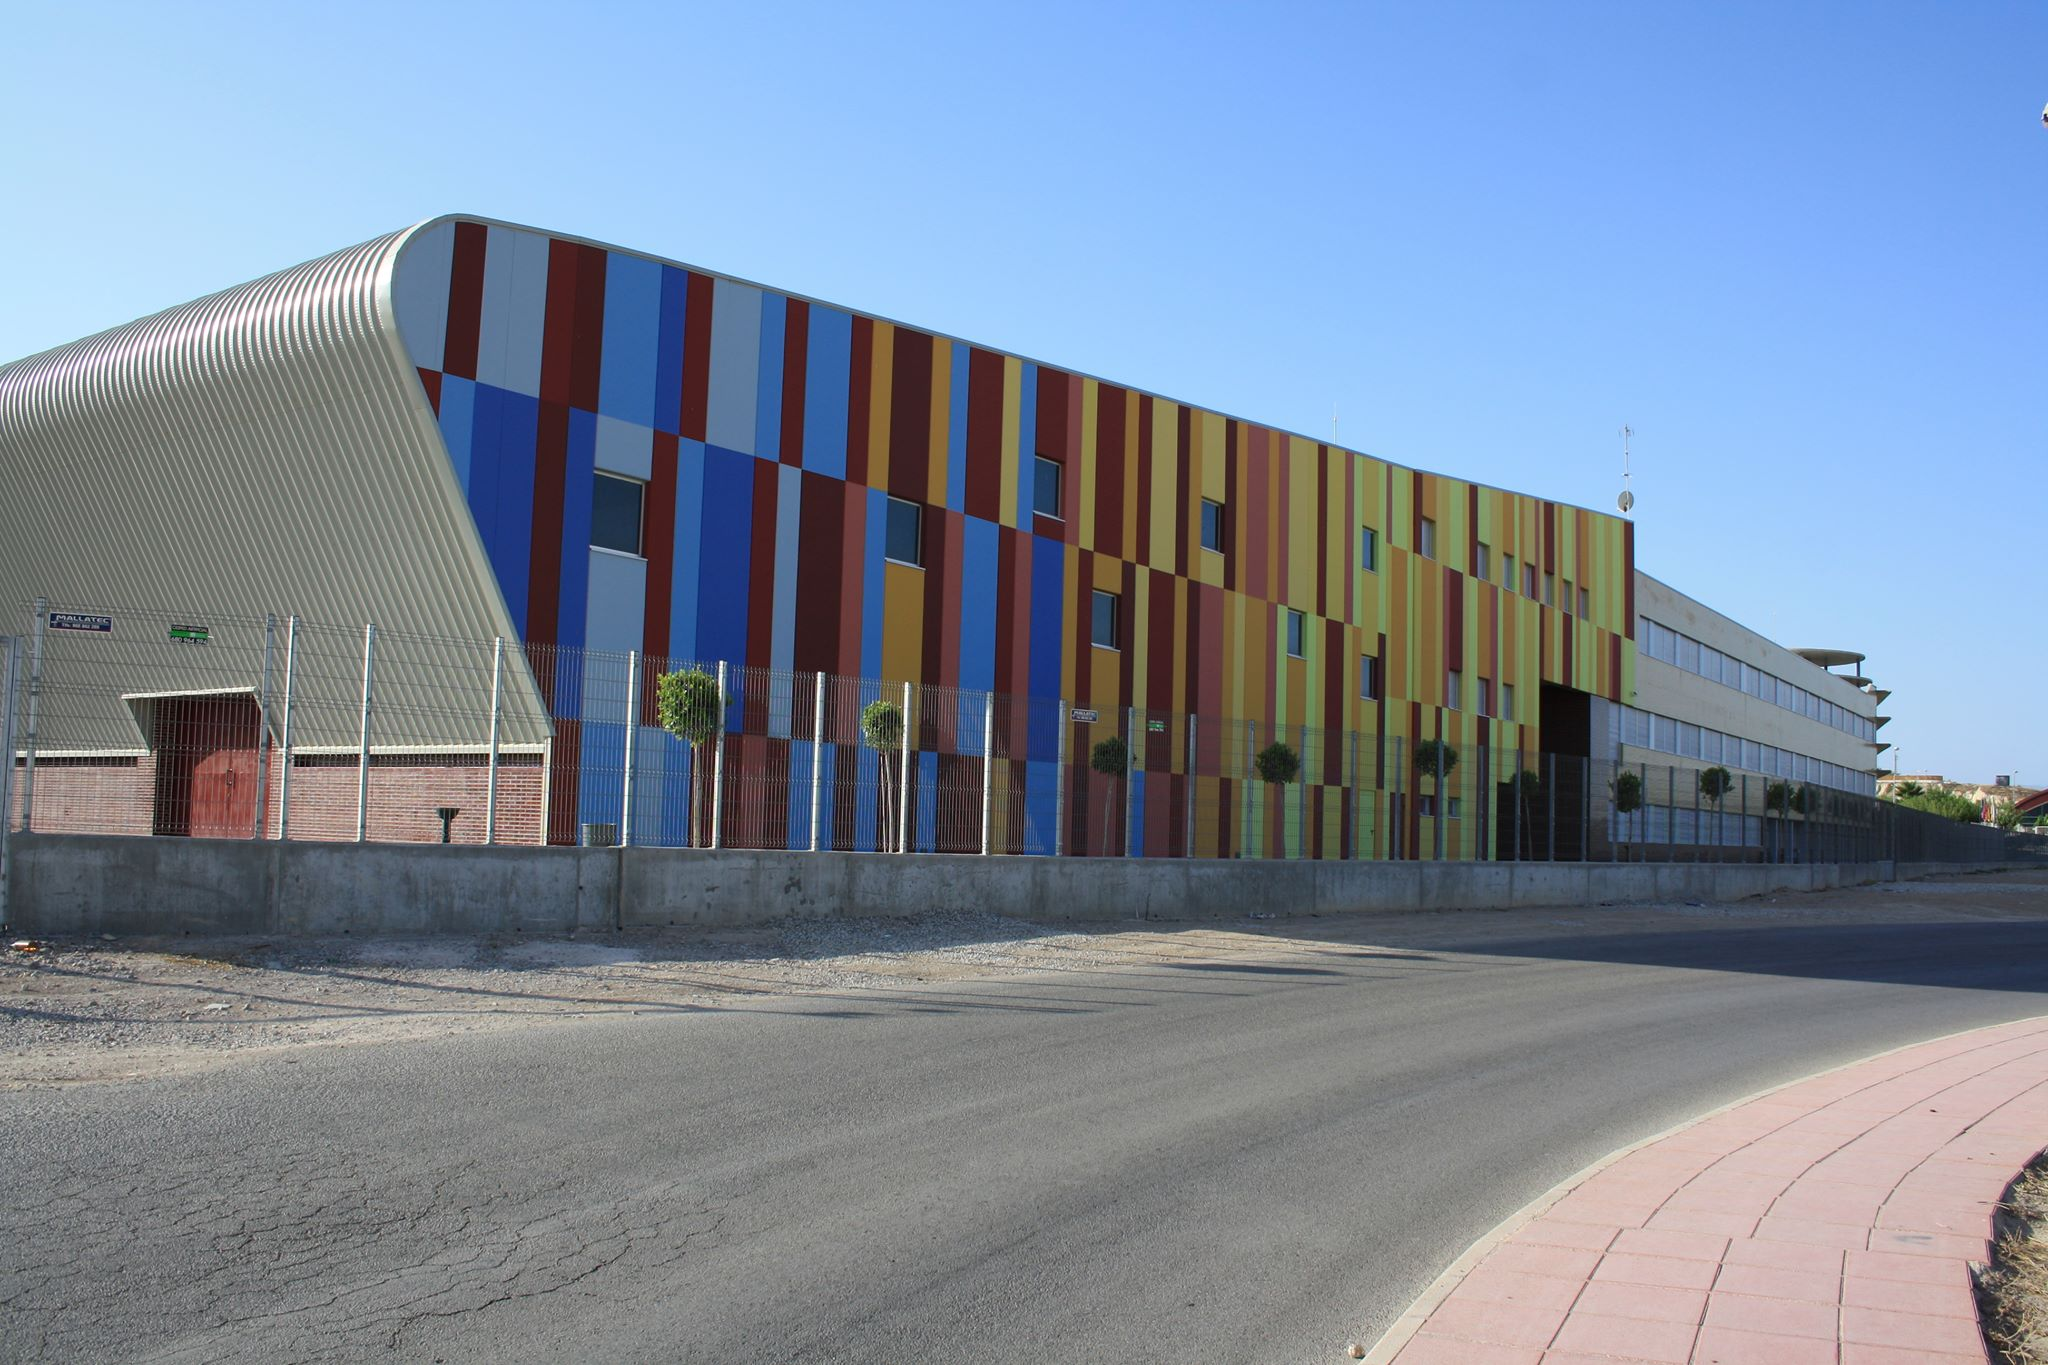
\includegraphics[width=.9\linewidth]{images/EduardoLinares}
  \caption { }
  \label{fig:pabellonFuera}
\end{subfigure}%
\begin{subfigure}{.5\textwidth}
  \centering
  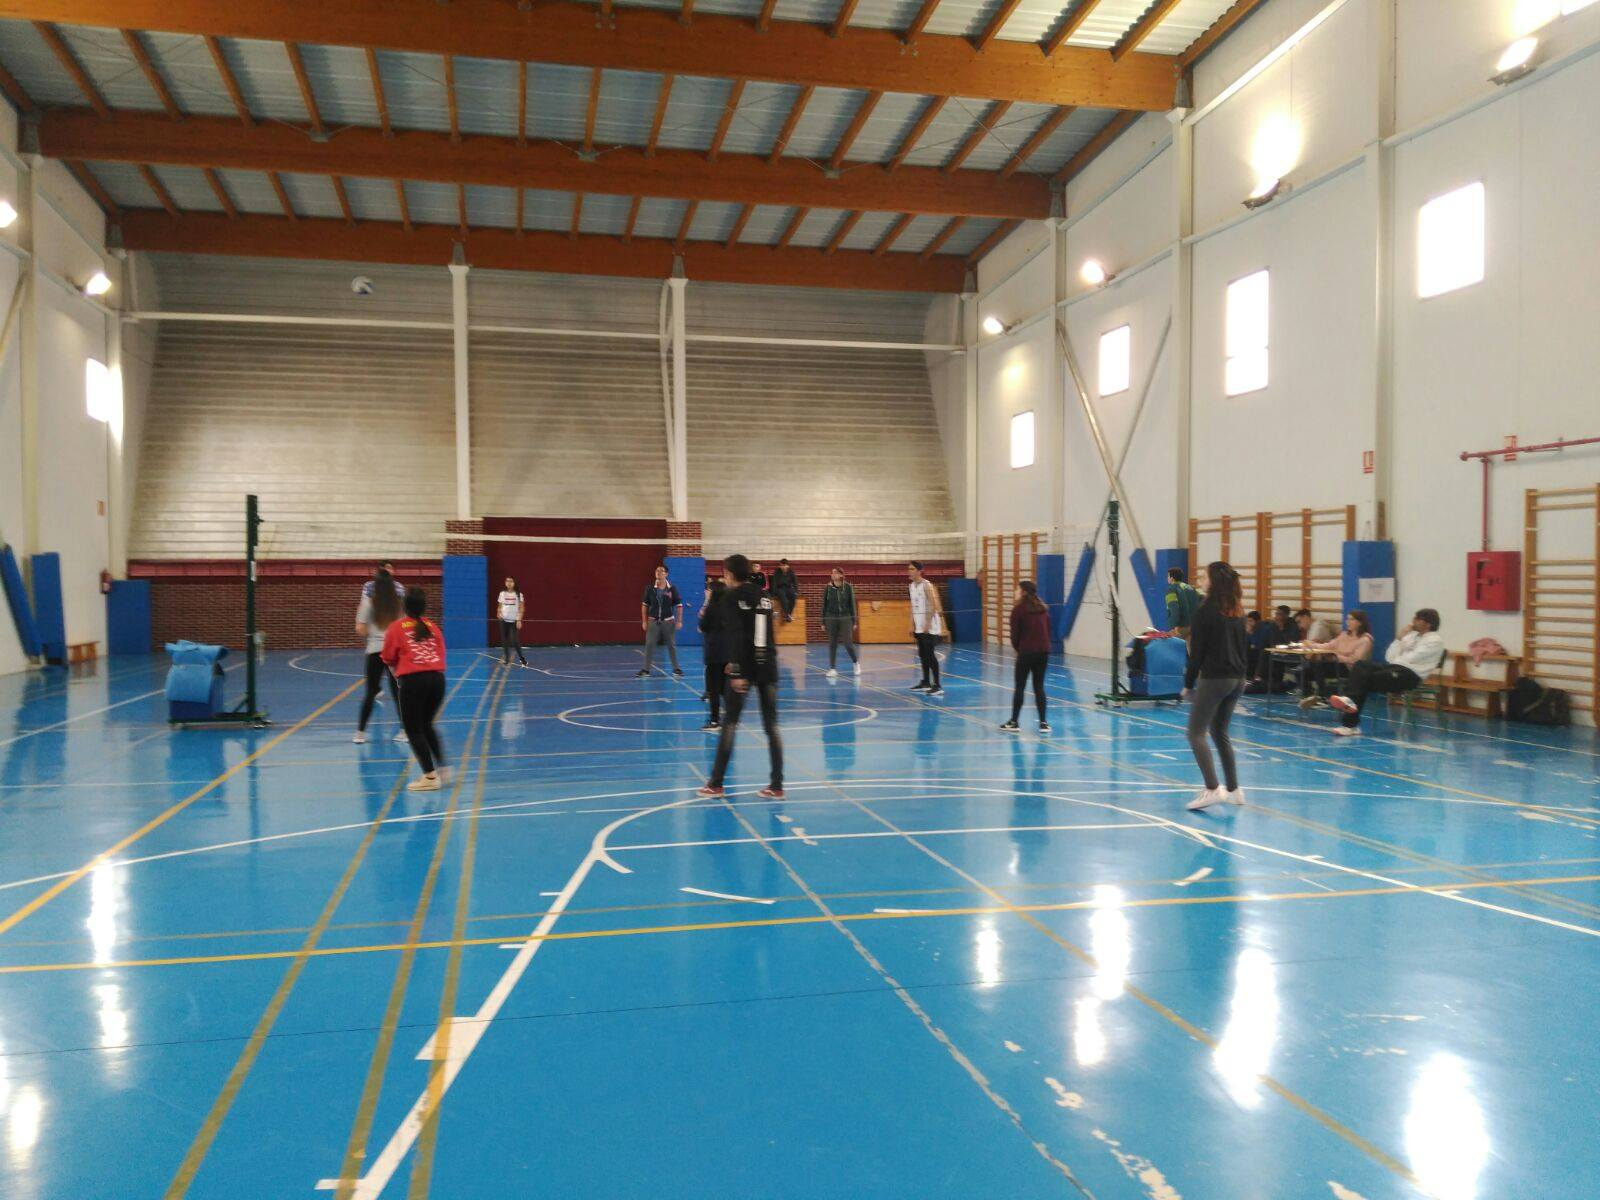
\includegraphics[width=.9\linewidth]{images/EduardoLinaresDentro}
  \caption { }
  \label{fig:pabellonDentro}
\end{subfigure}
\caption{Fotos del exterior (a) y del interior (b) del pabellón Eduardo Linares. }
\label{fig:pabellon}
\end{figure}

El pabellón en el que se instaló la cámara, previo permiso del Ayuntamiento, es el Eduardo Linares, en Molina de Segura, perteneciente al instituto de Enseñanza Secundaria Eduardo Linares, donde entrenan habitualmente las jugadoras del Club Molina Volley (figura \ref{fig:pabellon}).


\subsection{Herramientas utilizadas}
Durante la realización de este trabajo se han utilizado las herramientas listadas a continuación.

\subsubsection*{Python}

Python es un lenguaje de programación interpretado, multiparadigma y de tipado fuerte aunque dinámico. Nace a finales de los 80, pero alcanzó una mayor popularidad a partir de mediados de los 2000, poco después de la versión 2.0 del lenguaje. 

Con el tiempo, Python se ha convertido en uno de los lenguajes más utilizados en materia de procesado científico y \textit{machine learning}, debido a la sencillez con la que se puede programar en él, así como la disponibilidad de un gran abanico de librerías. Este último factor, unido a una mejor infraestructura para el despliegue de aplicaciones lo ha hecho más utilizado que su competidor más cercano, R.

La selección de Python como lenguaje para este proyecto está, por tanto, más que justificada ya que utilizaremos técnicas de \textit{deep learning}. Además las 2 librerías más importantes del proyecto (TensorFlow y OpenCV) se encuentran en Python.

\subsubsection*{Git}

Git es una herramienta de control de versiones originalmente desarrollada por Linus Torvalds para mantener el kernel de Linux. Su desarrollo comienza en abril de 2005 y su primera versión estable se lanzó en diciembre de ese mismo año. Poco a poco ha ido desbancando a Subversion, su competidor directo, como el software de control de versiones (VCS) más popular del mundo en la comunidad de desarrolladores debido a su gran potencia y flexibilidad.

En mi opinión, el software VCS es un requisito indispensable para cualquier proyecto de software, por la versatilidad que este aporta, desde ver el histórico de cambios en un proyecto como a la posibilidad de volver hacia atrás en caso de que en al desarrollar una parte de la aplicación algo haya ido mal. Además, en equipos cobra mayor importancia al permitir que dos personas trabajen sobre el mismo documento en apartados distintos a la vez que permitir una forma sencilla de compartir el código entre todos los miembros del equipo. En resumen, es difícil concebir un proyecto de software que no haga en absoluto empleo de este tipo de herramientas.

Para este trabajo ha sido utilizado como histórico de versiones a la vez que como forma de supervisar el código por parte de los directores.

\subsubsection*{OpenCV}

OpenCV (Open Source Computer Vision Library) es, como su nombre indica, una librería de código abierto orientada a visión por computador y \textit{machine learning}. Su objetivo es proporcionar una infraestructura común para aplicaciones de visión por computador, y dada su licencia BSD, es utilizada por empresas como Google, Microsoft o Intel, entre otras, para aplicaciones comerciales.

El desarrollo de la librería comienza en 1999 con un proyecto lanzado por Intel Research para proveer de una base de código estandarizada y optimizada para tareas de visión por computador. Tras una alfa lanzada en el 2000 en el IEEE Conference on Computer Vision and Pattern Recognition y sucesivas betas lanzadas entre 2001 y 2005, la librería alcanza su versión 1.0 en 2006. En la actualidad, OpenCV tiene más de 2500 algoritmos que mezclan una extensiva lista entre algoritmos clásicos y otros vigentes \cite{opencv}.

Aunque desarrollada nativamente en C++, OpenCV cuenta con un \textit{wrapper} para Python, el cual se utilizará para obtener imágenes de entrenamiento para el modelo a desarrollar, utilizando la base de código presente en mi TFG.

\subsection*{TensorFlow}

En 2011, Google Brain creó un sistema de \textit{machine learning} basado en redes neuronales, llamado DistBelief. Este sistema fue creciendo en el seno de la compañía tanto en aplicaciones comerciales como en investigación. Google acabó por pedirle a Jeff Dean entre otros que simplificaran la base de código existente en DistBelief, que acabaría por conocerse como TensorFlow, lanzando su primera versión en 2017 \cite{TensorFlow2015-whitepaper}.

La competencia durante los años siguientes fue dura con PyTorch, la alternativa desarrollada por Facebook. Cuando la investigación empezó a declinarse a favor de PyTorch, Google anunció una segunda gran versión de TensorFlow, con una gran cantidad de mejoras en cuanto a eficiencia y sencillez en desarrollo. 

En la actualidad ha acabado por convertirse en el framework de \textit{deep learning} más importante, con multitud de recursos e información disponibles para principiantes y expertos en la materia por igual. Un factor importante para el crecimiento de TensorFlow es la existencia de librerías auxiliares como Keras, que simplifican el código necesario para crear un modelo desde cero. Tal es la importancia de Keras que Google acabó por añadirla al core de TensorFlow y actualmente forma parte de este a la vez que se puede obtener en su versión \textit{standalone}.

Dado que en este proyecto desarrollaremos una red neuronal, TensorFlow/Keras será muy util para simplificar el código a escribir para obtener el modelo. Dado que el modelo será una CNN, será mejor utilizar la versión CUDA, que aprovecha el poder de procesamiento de las gráficas de Nvidia para cálculo matricial.

\newpage